% ---------------------------------------------------------------------
% Results --- compact 3-page version. Five key figures; the full 60-cell
% headline table is intentionally omitted (lives in the notebook output:
% report/tables/table_a_headline_30cells.{csv,tex}).
% ---------------------------------------------------------------------

\section{Results}
\label{sec:results}

The 60-cell run produced $241$ full solves out of $871$ executed
instances ($27.7\%$ pooled solve rate), with strong domain-tier
stratification (Section~\ref{sec:results:matrix}), a non-monotone
chain-of-thought effect (\ref{sec:results:cot}), a clean intra-family
scaling lift on most domains (\ref{sec:results:scaling}), and a
striking single-direction effect from reasoning post-training
(\ref{sec:results:qwq}). The full per-cell table appears in the
analysis notebook; this section walks through the five plots that
carry the headline findings.

\subsection{Domain-tier stratification}
\label{sec:results:matrix}

Table~\ref{tab:domain-rank} reports the pooled solve rate and mean
per-instance maximum \texttt{valid\_action\_\%} per domain.
Simple-tier domains (basic\_move, visit-all, satellite) cluster above
$74\%$ partial validity; complex-tier domains
(blocksworld, citycar, tetris) fall below $32\%$. The natural
breakpoint is between satellite ($75\%$ vap, $47\%$ solve rate) and
blocksworld ($32\%$ vap, $9.5\%$). The calibration is consistent with
the planner-derived reference plan lengths --- simple domains have
mean optimal plans $4.2$--$9.8$ actions; blocksworld reaches $26$ ---
suggesting an effective ceiling around the $\sim$8-action mark for
pure-token planning under our prompting and iteration setup.

\begin{table}[h]
\centering\small
\begin{tabular}{lrr}
\toprule
domain & solve rate & mean max vap \\
\midrule
\texttt{basic\_move}   & 89.0\% & 93.2\% \\
\texttt{visit-all}     & 85.0\% & 92.8\% \\
\texttt{satellite}     & 47.0\% & 74.8\% \\[2pt]
\texttt{blocksworld}   &  9.5\% & 31.9\% \\
\texttt{citycar}       &  0.5\% & 17.5\% \\
\texttt{tetris}        &  0.0\% & 13.6\% \\
\bottomrule
\end{tabular}
\caption{Domain difficulty pooled across all $5$ models and both
conditions.}
\label{tab:domain-rank}
\end{table}

\begin{figure}[h]
\centering
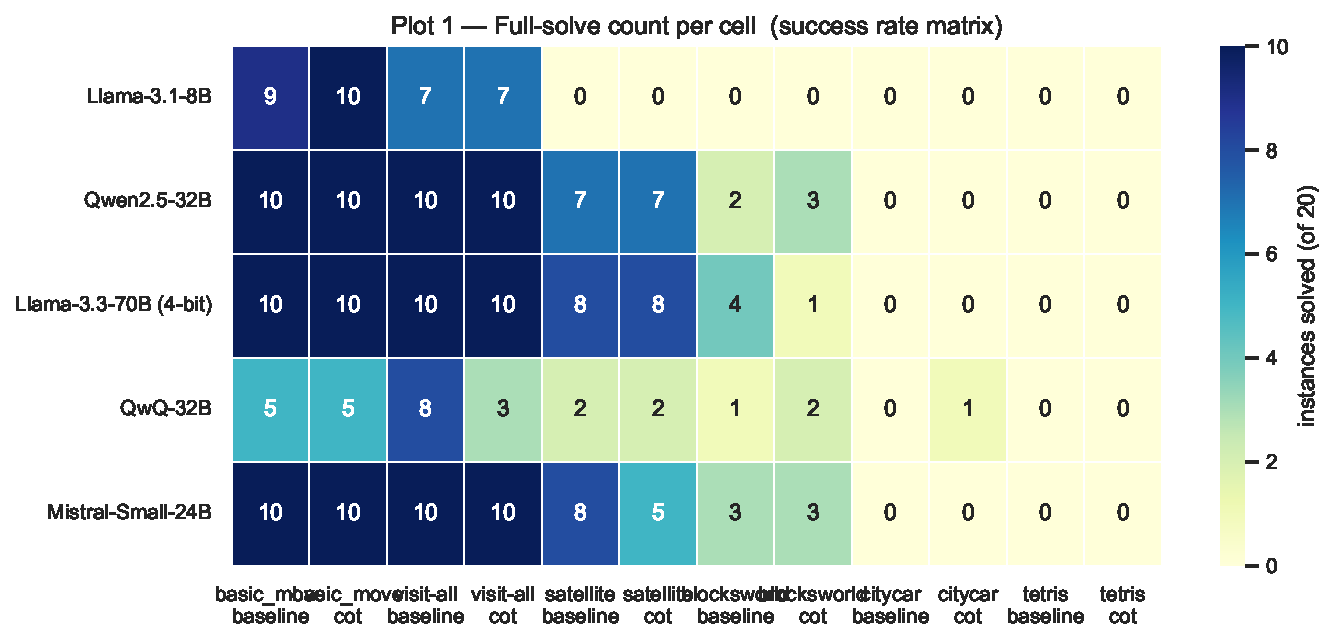
\includegraphics[width=0.92\textwidth]{figures/plot1_solves_heatmap.pdf}
\caption{Per-cell full-solve count out of $n$ instances ($n=10$ for
simple, $n=20$ for complex). Simple-domain columns saturate; complex
columns hover near zero except blocksworld.}
\label{fig:plot1}
\end{figure}

The granular picture (Figure~\ref{fig:plot2}) is mean per-instance
maximum partial validity. This view distinguishes models even where
the binary solve rate is zero: \texttt{qwen25}/citycar/baseline reaches
$45\%$ partial validity (almost-right plans) without ever hitting
$100\%$, whereas \texttt{llama33}/tetris/baseline produces plans
that VAL parses as $0\%$ valid throughout. The cumulative-solve curves
in Figure~\ref{fig:plot3} confirm that on the few cells where the
validator-feedback loop does meaningful work
(notably \texttt{llama33}/blocksworld/baseline, mean first-valid
iteration $2.5$) it lifts solve rate by a few percentage points across
iterations $2$--$4$; on most cells the iteration-1 column dominates
or no solves occur at all.

\begin{figure}[h]
\centering
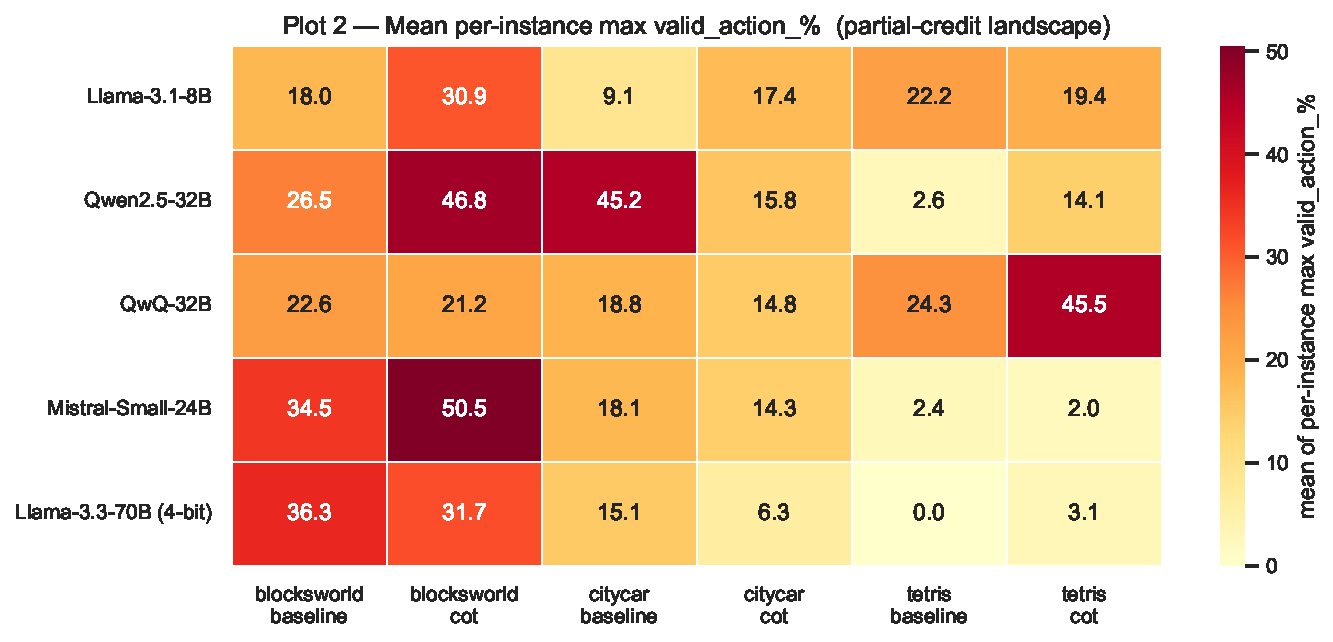
\includegraphics[width=0.92\textwidth]{figures/plot2_vap_heatmap.pdf}
\caption{Mean per-instance best \texttt{valid\_action\_\%}, the
partial-credit landscape.}
\label{fig:plot2}
\end{figure}

\begin{figure}[h]
\centering
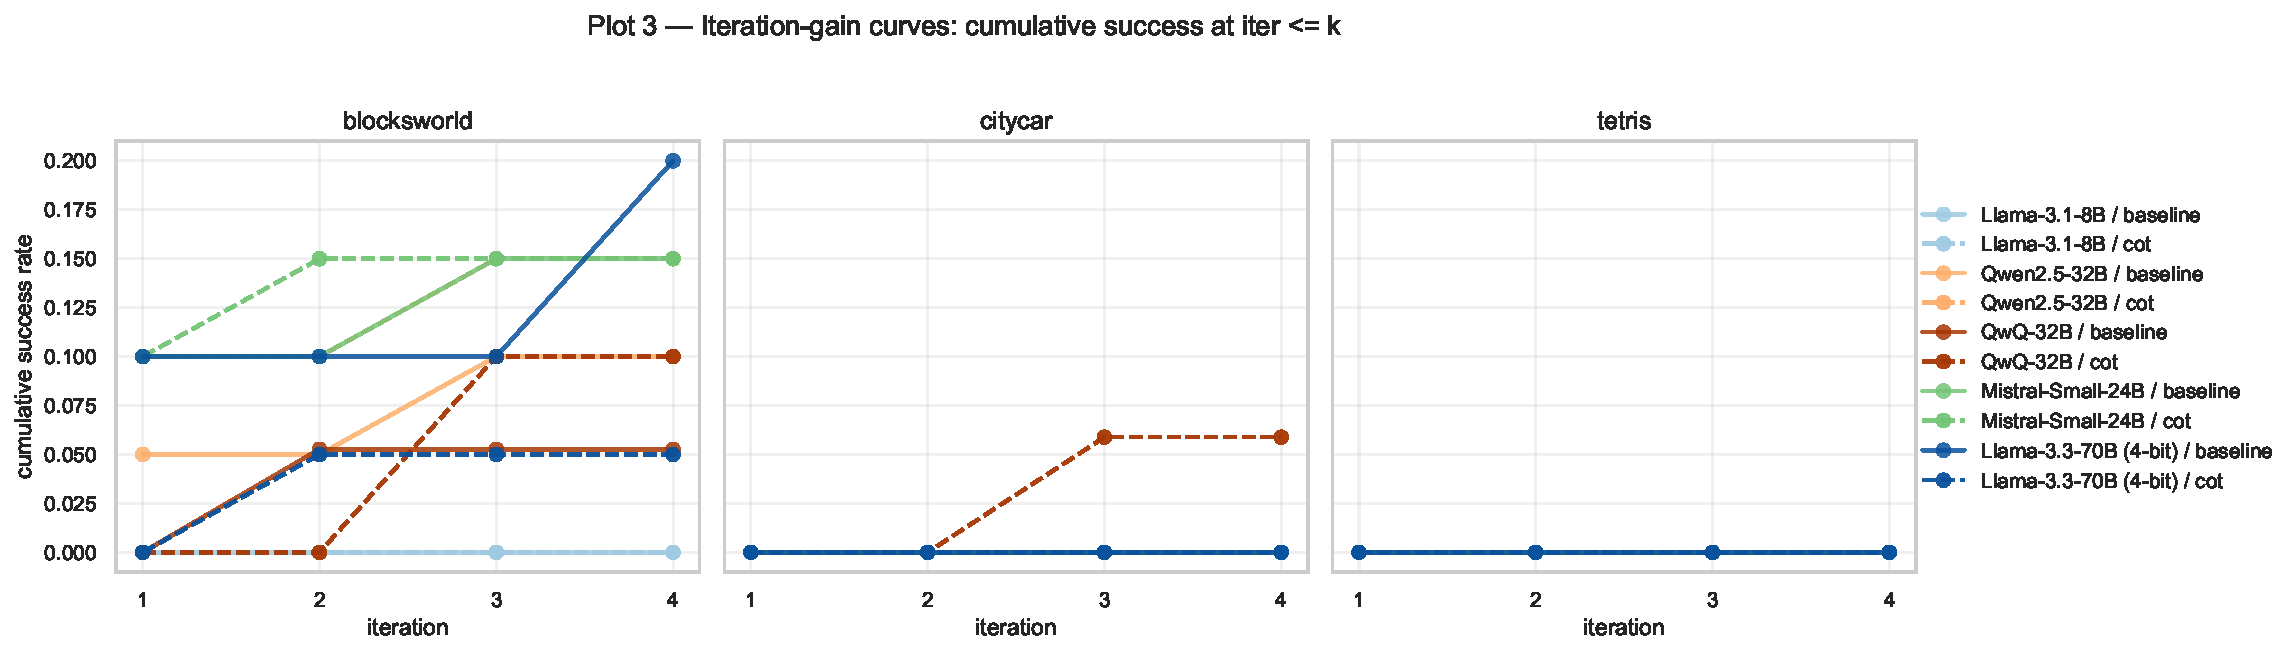
\includegraphics[width=0.92\textwidth]{figures/plot3_iteration_gain.pdf}
\caption{Cumulative success rate at iteration $\leq k$, one panel per
domain. Lines distinguish model and condition (solid = baseline,
dashed = cot).}
\label{fig:plot3}
\end{figure}

\subsection{Chain-of-thought effect}
\label{sec:results:cot}

CoT was the only deliberate prompt-axis manipulation. Across the $30$
\mbox{(model, domain)} pairs, $9$ show $\Delta\,\text{vap} > 1$~pp
(CoT helps), $13$ show $\Delta\,\text{vap} < -1$~pp (CoT hurts), and
$8$ are within $\pm 1$~pp (Figure~\ref{fig:plot4}). The pattern
correlates with domain difficulty: on the simple tier, CoT mostly
hurts because the reasoning preamble adds noise rather than structure
(e.g.\ \texttt{qwq32}/visit-all drops from $80\%$ to $30\%$ solve
rate). On blocksworld, CoT helps the smaller and mid-size models
substantially: \texttt{llama8} from $18.0\%$ to $30.9\%$ vap;
\texttt{qwen25} from $26.5\%$ to $46.8\%$;
\texttt{mistral24} from $34.5\%$ to $50.5\%$. There is no model for
which CoT is uniformly beneficial across all six domains.

\begin{figure}[h]
\centering
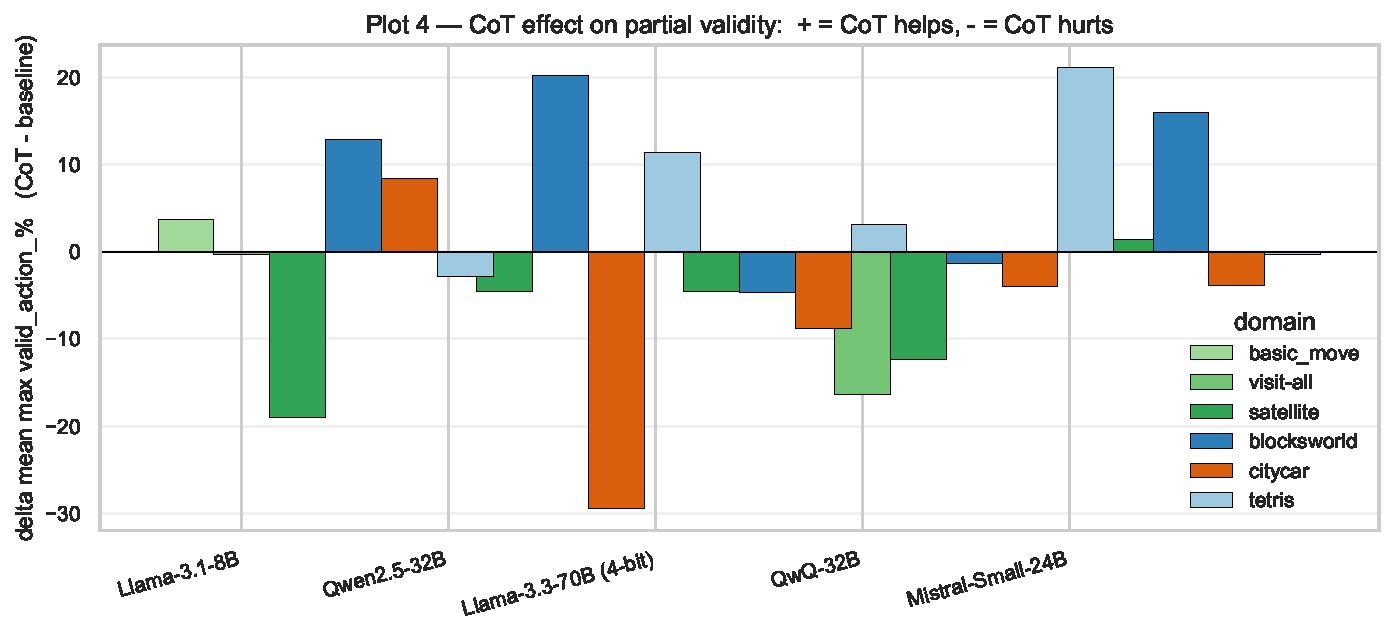
\includegraphics[width=0.92\textwidth]{figures/plot4_cot_delta.pdf}
\caption{$\Delta$ mean max \texttt{valid\_action\_\%} =
$\text{cot} - \text{baseline}$ per (model, domain) pair.
Bars above zero: CoT helps. Below zero: CoT hurts.}
\label{fig:plot4}
\end{figure}

\subsection{Intra-family scaling: Llama 8B vs.\ 70B}
\label{sec:results:scaling}

Pooled across the $12$ Llama cells, Llama-3.3-70B (4-bit) edges
Llama-3.1-8B (bf16) by $+10$~pp on partial validity ($57.2\%$ vs
$47.2\%$). The lift is concentrated on the simple-tier
\texttt{satellite} domain ($+30$~pp) and on \texttt{blocksworld}
baseline ($+18$~pp); on \texttt{tetris} the 70B model is actually
worse, reaching $0\%$ on baseline. Read this as: $4$-bit quantization
noise eats the partial-validity gain of three-fold parameter scaling
on the hardest domains. The bf16 70B comparison would have isolated
the scaling signal cleanly but did not fit on $2 \times$ A100-64\,GB.

\subsection{Reasoning-post-training ablation: QwQ-32B vs.\ Qwen2.5-32B}
\label{sec:results:qwq}

QwQ-32B is the same Qwen2.5 base architecture and parameter count with
reasoning post-training (RLHF + chain-of-thought traces) added.
Comparing the two models cell-by-cell isolates the post-training axis.
Figure~\ref{fig:plot7} shows that QwQ \emph{loses} on $9$ of $12$
cells, ties on $1$, and wins on $2$ (\texttt{tetris}/baseline and
\texttt{tetris}/cot --- the only domain where every model is bad).
Pooled $\Delta\,\text{vap} = -16.4$~percentage points. This is the
single largest model-level effect we observed and goes the
\emph{opposite} direction from what one might expect: the
reasoning-trained model is worse at PDDL planning than its base.
The likely mechanism is that reasoning post-training optimises for a
verbose \texttt{<think>...</think>} chain-of-thought style that
hurts structured-output tasks. The same long reasoning traces
caused $5$ of $12$ \texttt{qwq32} cells to TIMEOUT mid-iteration on
the $10$-hour walltime, censoring some data --- discussed in
Section~\ref{sec:limitations}.

\begin{figure}[h]
\centering
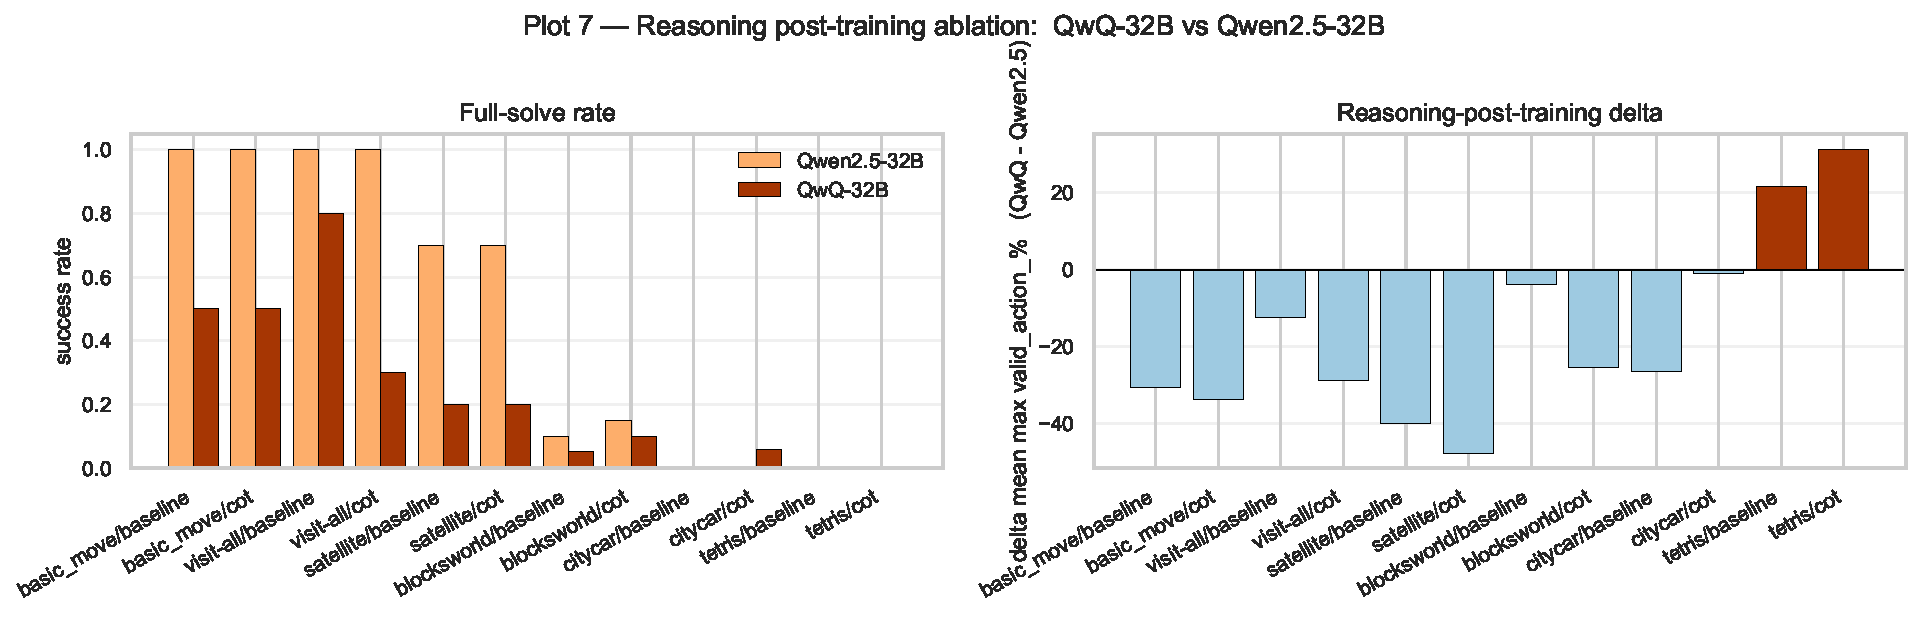
\includegraphics[width=0.92\textwidth]{figures/plot7_qwq_ablation.pdf}
\caption{Reasoning-post-training ablation. Left: full-solve rates side
by side per cell. Right: $\Delta$ mean max \texttt{valid\_action\_\%}
$= \text{QwQ} - \text{Qwen2.5-32B}$. Negative bars: reasoning training
hurts.}
\label{fig:plot7}
\end{figure}

\subsection{Per-instance difficulty calibration}
\label{sec:results:per-instance}

Cross-referencing the planner-derived reference plan lengths with
empirical per-instance partial validity (Figure~\ref{fig:plot15})
shows a meaningful negative slope and Pearson correlation across the
four domains where reference plans exist: harder problems in the
formal-planner sense really are harder for LLMs, in the same direction
and roughly the same magnitude. This rules out the worry that LLM
scores are noise on the difficulty axis and validates the cross-domain
ranking implied by Table~\ref{tab:domain-rank}.

\begin{figure}[h]
\centering
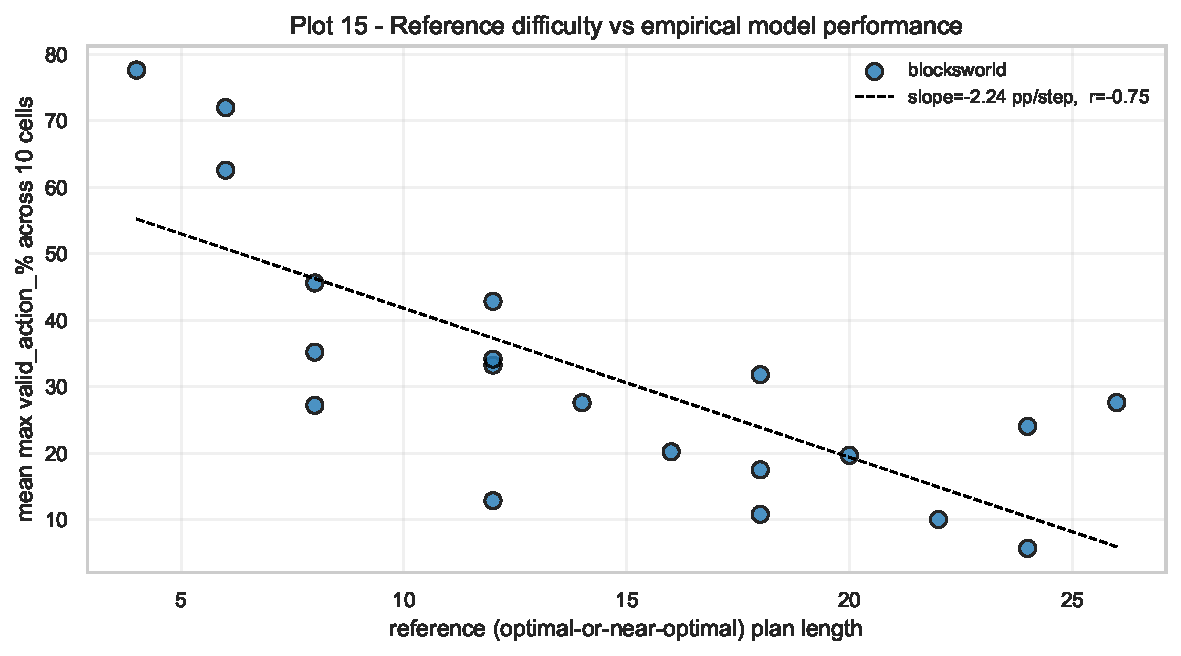
\includegraphics[width=0.78\textwidth]{figures/plot15_difficulty_vs_performance.pdf}
\caption{Reference difficulty (x: optimal plan length) vs.\ empirical
model performance (y: mean per-instance max \texttt{valid\_action\_\%}
across $10$ \mbox{(model, condition)} cells). One point per
\mbox{(domain, instance)}. Black dashed: OLS fit; legend reports
slope and Pearson $r$.}
\label{fig:plot15}
\end{figure}

The notebook's full set of $15$ figures (per-iteration token
distributions, first-valid-iteration stack, partial-credit boxplots,
per-instance consensus difficulty, and others) is preserved under
\texttt{report/figures/} for readers who want a deeper view than the
five headline plots reproduced here.
